\documentclass{article}
\usepackage{hyperref}
\usepackage[utf8]{inputenc}
\usepackage{amsfonts}
\usepackage{amsmath}
\usepackage{amssymb}
\usepackage{tikz}
\usepackage{bbm}
\usepackage{relsize}
\usepackage{pgfplots}
\usepackage{scalerel}
\usepackage{wrapfig}
\usepackage[T1]{fontenc}       % change font encoding to T1
\usepackage[framed,numbered]{matlab-prettifier}
\pgfplotsset{width=10cm,compat=1.9}
\addtolength{\oddsidemargin}{-.875in}
	\addtolength{\evensidemargin}{-.875in}
	\addtolength{\textwidth}{1.75in}

	\addtolength{\topmargin}{-.875in}
	\addtolength{\textheight}{1.75in}

\title{Meccanica Razionale Riassunti}
\author{Simone Paloschi}
\date{terzo Anno primo Semestre INGMTM}
\linespread{1.5}

\begin{document}


%
%
Oss: Siano $\overline{\omega}(t)$ la velocità angolare di $\theta'$ rispetto a $\theta$ e $\overline{\omega}'(t)$ quella di $\theta$ rispetto a $\theta'$ allora $\dot{\overline{\omega}} = \dot{\overline{\omega}'}$ \\ \\ \\
%
%
Analizziamo ora la riduzione dei gradi di libertà per i \textbf{vincoli} più frequenti: \ \ \ \ \ \ \ \ \ \ \ \ \ \
%
\begin{wrapfigure}{l}{0.17\textwidth}
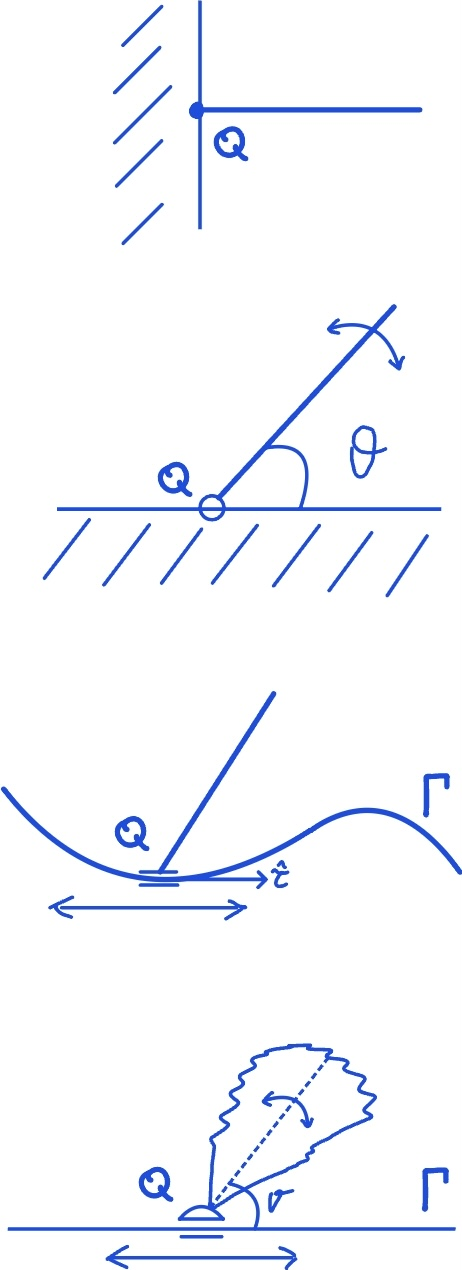
\includegraphics[width=0.17\textwidth]{Vincoli.jpeg}
\end{wrapfigure} \\
%
%
\textbf{Incastro} \ \ $\overline{x}_Q(t)=\overline{x}_P(t)$\\
Il corpo non si muove rispetto a Q \ \ \ \ g= g$_0$-g$_0$ =0\\ \\
%
%
\textbf{Cerniera} fissa e mobile \ \ \ \ $\overline{x}_{Q_1}(t)=\overline{x}_{Q_2}(t) \ \Leftrightarrow \ \overline{V}_{Q_1}(t)=\overline{V}_{Q_2}(t)$ e integrabile \linebreak
Moto e Atto rotatorio con asse di i.r. passante per Q e \ \ g =$\begin{cases} g_0 -2 \ \ se \ d=2 \\ g_0 -3 \ \ se \ d=3 \end{cases}$\\ \\
%
%
\textbf{Manicotto} \ \ $\overline{v}_P(t) = v_P \hat{\tau}_P(t) \ \ \forall P$ appartenente al corpo \\
Non si ha moto del corpo relativo a Q \ \ e quindi \ g =$\begin{cases} g_0 -2 \ \ se \ d=2 \\ g_0 -4 \ \ se \ d=3  \end{cases}$\\ \\
%
%
\textbf{Carrello} \ \ $\overline{v}_Q(t) = v_Q \hat{\tau}_Q(t) \ \ \forall Q \in \Gamma$ \ \ \ \ \  g =$\begin{cases} g_0 -1 \ \ se \ d=2 \\ g_0 -2 \ \ se \ d=3  \end{cases}$\\ \\
In d=2: cerniera fissa genera moto rotatorio e manicotto  genera moto traslatorio \linebreak \\ \\ \\
%
%
%
\textbf{Tipi di vincoli ideali:}\\
%
\ • \ Guida perfetta (in assenza di attrito) \ \ $\overline{\Phi} = \overline{\Phi}_n \hat{n}(s)$ \ \ (perché $\delta\overline{x}_P'=\mu\hat{\tau}(s)$) \\
%
\ • \ Incastro perfetto \ $(\overline{\Phi}, C) \ \overline{M}_C$ \ (perché $\overline{v}_P'=\overline{0} \ \forall P \implies \Phi$ qualsiasi e serve $\overline{M}$ per contrastare rotazioni)\\
%
\ • \ Appoggio ideale (senza attrito) \ \ $\overline{x}_P'=\Phi_n\hat{n}(s) \ \ \Phi_n\geq0$ \\ (perché $\delta \overline{x}_P'=\lambda\hat{i} + \mu \hat{j}$ con $\lambda\in\mathbb{R}, \ \mu\in\mathbb{R}^+$, allora preso $\mu =0$, per avere $\overline{\Phi}\cdot\overline{x}_P'\geq0 \ \forall \lambda$ serve $\Phi /\!\!/ \hat{j}$)\\
%
\ • \ Puro rotolamento $(\overline{\Phi},H) \ \ \overline{\Phi}=\Phi_{\tau}\hat{\tau}(s)+\Phi_n\hat{n}(s) \ \ \begin{cases}
\Phi_{\tau} \in \mathbb{R}, \Phi_n\in\mathbb{R}^+ \ \ (appoggio, \ \overline{v}_H'=\lambda\hat{j} \ \ \lambda \geq \overline{0}) \\
\Phi_{\tau}, \Phi_n \in \mathbb{R} \ \ (vincolo, \ \overline{v}_H'=\overline{0})
\end{cases}$ \\ \\
%
\ • \ Cerniera fissa perfetta \  $(\overline{\Phi},C)$ (perché $\overline{v}_C'=\overline{0}$) \ \ • \ Cerniera mobile perfetta \ $(\overline{\Phi}_1,C) (\overline{\Phi}_2,C)$ con $\overline{\Phi}_1=-\overline{\Phi}_2$ \\
%
\ • \ Manicotto perfetto e Carrello perfetto \ \ \ $(\overline{\Phi},C) \ \ \overline{\Phi}=\Phi_n\hat{n}(s)$ \ \ (inoltre manicotto 2D serve $\overline{M}_C /\!\!/ \hat{k}$) \\ \\ \\
%
%
%
%

\end{document}